\chapter{Introdução}
\label{chap:introdução} 

\section{Contexto}

Segundo\cite{WillcocksTercerizacao} a terceirização do desenvolvimento de software é uma prática cada vez mais adotada por organizações. A terceirização de atividades, ou seja, o ato de transferir para fora da organização uma parte do seu processo produtivo, não é uma prática recente. Atividades e processos que eram muito específicos dentro de uma organização foram transferidos, de forma parcial ou total, para outras organizações ou agentes externos \cite{leite_terceirizacao}.

Uma das motivações para a terceirização é a qualidade do serviço prometida pelas empresas fornecedoras. No entanto, existem vários riscos associados à decisão pela terceirização, que podem comprometer a qualidade esperada, como por exemplo: as expectativas de serviço e a resposta rápida não serem atendidas adequadamente; o serviço prestado apresentar qualidade inferior ao existente anteriormente; e as tecnologias utilizadas não corresponderem ao esperado\cite{WillcocksTercerizacao}. Segundo\citeonline{GuiaAquisicao} a aquisição de um \textit {software} é um processo complexo, principalmente no que diz respeito à caracterização dos requisitos necessários ao \textit {software} e às condições envolvidas na contratação como a qualidade esperada. 
 
Acompanhando o ritmo da terceirização o cenário com empresas terceirizadas contratadas para o desenvolvimento de \textit {software} está cada vez maior em organizações públicas. Tais organizações não são diretamente responsáveis pelo desenvolvimento do \textit {software} mas são responsáveis  pelo processo de verificação de sua qualidade conforme a norma \citeonline{Normativa4} que será explicada no capítulo \ref{chap:contratos} deste trabalho. \textcolor{red}{Arrumar essa referência no BBTec. Deveria aparecer IN4/2008 e nao Brasil}




\section{Justificativa}

Segundo \cite{beck1999}\cite{fowler1999refactoring} a qualidade de \textit{software} é medida pela qualidade de seu código-fonte. Conforme a \cite{ISO:15939} medição é uma ferramenta primordial para avaliar a qualidade dos produtos e a capacidade de processos organizacionais, portanto o Órgão Público contratante pode fazer uso do monitoramento de métricas de código-fonte para assistir ao processo de aferição de qualidade do \textit{software} desenvolvido pela contratada.

\cite{rego_monitoramento_2014} propôs uma solução para o monitoramento de métricas de código-fonte com suporte de um ambiente de \textit{Data Warehousing} que será explicada no capítulo 5. Uma das principais contribuições deste trabalho será evidenciar a eficácia e a eficiência da proposta por \citeonline{rego_monitoramento_2014} na aferição da qualidade do software adquirido de uma empresa terceirizada para equipe responsável da organização pública e seus demais envolvidos.

\section{Problema}
\label{sec:problema} 

Com foco na avaliação de controles gerais de Tecnologia da Informação nos órgãos públicos, em 2011, o Tribunal de Contas da União-TCU detectou, por meio de auditorias de governança de TI, em diversos órgãos uma considerável frequência de irregularidades relacionadas à inexistência, deficiências e a falhas de processos de \textit{software} que comprometem a eficácia e eficiência das contratações de desenvolvimento de sistemas \cite{Acordao381_2011}. 

A inexistência de parâmetros de aferição de qualidade para contratação de desenvolvimento de sistemas e a deficiência no processo de contratação, decorrente da inexistência de metodologia que assegure boa contratação de desenvolvimento de sistemas foram listados nas auditorias como consequências da inexistência e falha de processos de \textit{software} nos órgãos públicos. Os critérios indicados pelo TCU no acórdão \cite{Acordao381_2011} foram:Constituição Federal, art. 37, caput; Instrução Normativa 4/2008, SLTI/MPOG, art. 12, inciso II; Lei 8666/1993, art. 6º, inciso IX; Norma Técnica - ITGI - Cobit 4.1, PO8.3 - Padrões de desenvolvimento e de aquisições; Norma Técnica - NBR ISO/IEC - 12.207 e 15.504;e Resolução 90/2009, CNJ, art. 10. 

A auditoria do acordão \cite{Acordao381_2011} reforça o problema da falta de capacidade da administração pública de aferir a qualidade interna dos produtos de software desenvolvido por terceirizadas. A partir desse problema e da solução para monitoramento de métricas de código-fonte com suporte de um ambiente de \textit{Data Warehousing-DWing} proposta por \citeonline{rego_monitoramento_2014} , foi formulada a questão de pesquisa geral deste trabalho que é:

\textbf{O uso de DW para o monitoramento de métricas de código fonte para assistir ao processo de aferição de qualidade interna dos produtos de software desenvolvido por terceirizadas, do ponto de vista da equipe de qualidade software de uma empresa pública, é eficaz e eficiente?}


\section{Objetivos}

O objetivo geral deste trabalho é realizar um estudo de caso onde será analisada
a eficácia e a eficiência do uso de um ambiente de DWing para o monitoramento de métricas de código fonte de forma a assistir ao processo de aferição de qualidade interna dos produtos de software desenvolvidos por uma organização terceirizada, por parte de uma organização pública. Dentre os objetivos específicos deste trabalho estão:

\begin{easylist}[itemize]
& Levantar fundamentação teórica que servirá de base para todo o trabalho.

& Apresentar solução desenvolvida por \citeonline{rego_monitoramento_2014} para monitoramento de métricas através de \textit{Data Warehousing}. 

& Definir, projetar e caracterizar o do estudo de caso.

& Criar novos cenários de limpeza de código-fonte, em estensão a solução proposta por \citeonline{rego_monitoramento_2014}.  

& Construir um \textit{dashboard}, com auxílio das ferramentas descritas no capítulo \ref{chap:arquitetura},  para dar maior visibilidade para as métricas e cenários de limpeza. 

& Coletar os dados que surgirão como respostas das questões específicas elaboradas para o estudo de caso, como por exemplo o nível de satisfação quanto ao uso da solução ou qual a taxa de oportunidade de melhoria de código em um determinado intervalo de tempo.

& Coletar métricas e cenários de limpeza a partir código-fonte do \textit{software} adquirido pela organização selecionada.

& Realizar análise dos dados coletados.

& Relatar resultados obtidos.
	

\end{easylist}

\section{Metodologia de pesquisa}

O que é uma pesquisa? De acordo com \cite{gil_como_2002} é o procedimento racional e sistemático que tem como objetivo proporcionar respostas aos problemas que são propostos. A pesquisa é requerida quando não se dispõe de informação suficiente para responder ao
problema, ou então quando a informação disponível se encontra em tal estado de desordem que não possa ser adequadamente relacionada ao problema.

Nessa seção apresenta-se a metodologia de pesquisa adotada neste trabalho. Para
isso, foram definidos: a natureza da pesquisa; o tipo de metodologia de pesquisa; o tipo de abordagem de pesquisa; os métodos de procedimentos de pesquisa e os tipos de técnicas
de coletas de dados.

Os procedimentos de pesquisa selecionados foram pesquisa bibliográfica, documental, levantamento e estudo de caso. As técnicas de coleta de dados selecionadas foram
entrevistas, questionários e registro de observação na vida real. A seleção metodológica é apresentada na Figura \ref{7eixosqualidade} e a descrição das classificações adotadas se encontra na Tabela \ref{tab:descricaoMetodologia}.

\begin{figure}[h!]
\centering
\includegraphics[keepaspectratio=false,scale=0.5]{figuras/figuras_nilton/selecaoMetodologica.eps}
\caption{Metodologia de Pesquisa}
\label{7eixosqualidade}
\end{figure}

\begin{table}[!ht]
	\begin{center}
	
	\input{tabelas/tabelasNilton/tabelaDescricaoMetodologia.ltx} 
	\caption{Descrição das classificações adotadas de pesquisa, conceitos extraídos de  \citeonline{metodologia_edna}}
	\label{tab:descricaoMetodologia}
	\end{center}
	\end{table}	
	\FloatBarrier

Segundo \cite{yin2001estudo} o estudo de caso é um conjunto de procedimentos pré-especificados para se obter uma investigação empírica que investiga um fenômeno contemporâneo dentro de seu contexto da vida real, especialmente quando os limites entre o fenômeno e o contexto não estão claramente definidos. Uma grande vantagem do estudo de caso é a sua capacidade de lidar com uma ampla variedade de evidências - documentos, artefatos, entrevistas e observações - além do que pode estar disponível no estudo histórico convencional. Além disso, em algumas situações, como na observação participante, pode ocorrer manipulação informal.

\cite{wohlin2012experimentation} fraciona o estudo de caso em cinco passos. Nesta pesquisa, o estudo de caso compreende os passos: Planejar o Estudo de Caso; Coletar Dados; Analisar Dados Coletados e Compartilhar os Resultados. Portanto, os passos Projetar o Estudo de Caso e Preparar a Coleta de Dados definidas por \citeonline{wohlin2012experimentation} foram agrupadas no passo Planejar o estudo de caso como na Figura \ref{passo Estudo de Caso}.

\begin{figure}[h!]
\centering
\includegraphics[keepaspectratio=false,scale=0.5]{figuras/figuras_nilton/passosEstudoCaso.eps}
\caption{Passos do Estudo de Caso}
\label{passo Estudo de Caso}
\end{figure}

O passo Planejar o Estudo de Caso consiste na determinação do objetivo e da questão de pesquisa, da escolha da metodologia de pesquisa, da definição das fases da pesquisa, da definição do procedimentos de pesquisa, do protocolo, das técnicas de coleta de dados e da proposta do trabalho final.

No passo Coletar Dados são executados os procedimentos de pesquisa e as técnicas de coletas de dados a seguir:

\begin{easylist}[itemize]
& Pesquisa Bibliográfica: pesquisa realizada a partir de livros, dissertações e trabalhos relacionados à área de pesquisa;

& Pesquisa Documental: pesquisa realizada a partir de documentos publicados por organizações públicas;

& Estudo de Caso: utilizar um estudo de caso real de uma organização pública brasileira;

& Entrevistas: dados serão coletados por meio de entrevistas informais, além de questionário, para incremento do estudo de caso;

& Documentos: coleta de dados dos documentos dos processos fornecidos pelo órgão público do estudo de caso será realizada para coleta de dados para análise;

& Observação na Vida Real: coleta de dados a partir da observação no campo de estudo;

\end{easylist}

O passo Analizar Dados Coletados é onde os dados coletados serão analisados e interpretados. A análise compreende tanto a análise quantitativa quanto a análise qualitativa.

Por fim, o passo Compartilhar os resultados diz respeito expor os resultados de forma adequada para o leitor alvo.



\section{Organização do Trabalho}

Esse trabalho está dividido em 5 capítulos:

	\begin{easylist}[itemize]	
	
	& \textbf{Capítulo 1 - Introdução:} Esse capítulo tem como objetivo apresentar o contexto que esse trabalho está inserido, o problema sobre o qual ele buscará resolver, qual a justificativa, os objetivos da sua realização e metodologia de pesquisa adotada.
	& \textbf{Capítulo 2 - Métricas de Software:} Capítulo responsável pela explicação teórica a respeito do que são métricas de código e como elas foram utilizadas no desenvolvimento da solução que esse trabalho busca analisar.
	& \textbf{Capítulo 3 - Contratações de Fornecedores de Desenvolvimento de Software:} apresenta-se as principais informações referentes à Contratação de Fornecedores de Desenvolvimento de Software. Para isso, o capítulo é iniciado com uma visão geral sobre a importância das contratações e suas principais características. Posteriormente, é apresentado um resumo da Instrução Normativa 04.
	& \textbf{Capítulo 4 - Data Warehouse:} Nesse capítulo serão apresentados conceitos teóricos sobre \textit{Data Warehousing}, assim como a maneira como foi desenvolvido e como funciona o ambiente de \textit{Data Warehouse} para armazenamento de métricas de código fonte.
	& \textbf{Capítulo 5 - Projeto de estudo de caso:} é apresentado o projeto do estudo de caso resultante do passo planejar Estudo de Caso, buscando demonstrar o escopo e elaborar um protocolo para o estudo de caso que será realizado. Elementos de pesquisa serão identificados e explicados como o problema a ser resolvido, os objetivos a serem alcançados no estudo de caso, quais os métodos de coleta e a análise dos dados.
	& \textbf{Capítulo 6 - Conclusão:} Além das considerações finais dessa primeira parte do trabalho, serão descritos objetivos para o trabalho de conclusão de curso dois.
	\end{easylist}
